\chapter{Introduction}
\label{chapter:Introduction}
In the field of computer vison and pattern recognition, determining a
model from a finite set of samples or a complex image without a prior
knowledge is an ill-posed problem. Due to the the ill-posedness, in
the sense that a unique model may not exist, models specifying a prior
knowledge plays an very important role in solving many important
computer vision problems, such as object tracking, shape recognition,
pose estimation, segmentation, edge detection, stereo matching and 3-D
reconstruction.

Some parametric curve models, also known as deformable models,
deformable templates, snakes, or active contours, have been developed
to guide the image interpretation process towards particularly
likely interpretations~\cite{hanek2004fitting}. These parametric curve
models have had two outstanding influences on the
development of related algorithms. The first is the Snakes which
represent a fundamentally new framework for delineating an object
outline in an image. This algorithm attempts to minimize energy
associated to the current contour as a sum of an internal and an external
energy~\cite{kass1988snakes}. The goal of snakes is to balance the prior
knowledge with evidence from an image. The second outstanding
influence is in the field of pattern recognition and machine learning,
where statistical distributions plays a key role.  There treatment
of a prior knowledge about shape is put into a probabilistic
context. Any shape is regarded as the result of applying some
distortion to an ideal prototype shape, and an appropriate
distribution governs the nature and extent of that distortion.
For both kinds of methods, the common aim is to strengthen the visual
interpretation of the shape via the establishing influence of prior
expectations of the shapes that are likely to be
seen~\cite{blake1998active}. This thesis dwells upon the Contracting
Curve Density (CCD) algorithm whose basic step is solving a
curve-fitting problem in a probabilistic context.


\section{The CCD Algorithm and Curve-fitting Problem}
\label{sec:ccdcfp}
The curve-fitting is a process that makes
a practical deformable template (model) attached to the feature in a
image. In essence it involves using algorithms to find the parameter
values for a given parametric curve model. Lots of important and
challenging computer vision tasks can be formulated as variants of the
curve-fitting problem. 

Suppose we have an observed object in an
image. Boundaries of the object can be completely or partially defined
by an either open or closed curve obtained by human intervention or
some object recognition techniques, such as SIFT features or reconstruction. The goal of
curve-fitting problem is to accurately identify \textit{decision boundaries} (2-D) or
\textit{decision surfaces} (3-D)~\cite{bishop2006pattern} by
distorting the curve. Since the approximate boundaries of the observed
object have been been given by the prior curve, there is no need to organise or group features in the
image, and the analysis can be restricted to a relatively narrow
ROI (region of interest), as a result, performance of such algorithms
is boosted up. In the resulting ROI, we aim to distort the contour in a specific
shape-space and make it attach to the boundary of a given object. This
is a curve-fitting problem, and the CCD approach discussed in this
thesis is a powerful model-based algorithm to solve the curve-fitting
problem.

The CCD algorithm can be described as follows. Given one or multiple images as input
data and a parametric curve model with a prior distribution of model
parameters, through curve-fitting process we estimate the model
parameters which determine the approximation of the posterior
distribution in order to make the curve models best matching the image data.
Fig.~\ref{fig:fitting} depicts a curve-fitting problem, and the corresponding solution is obtained by the
CCD algorithm.
\begin{figure}[htb]
  \centering
  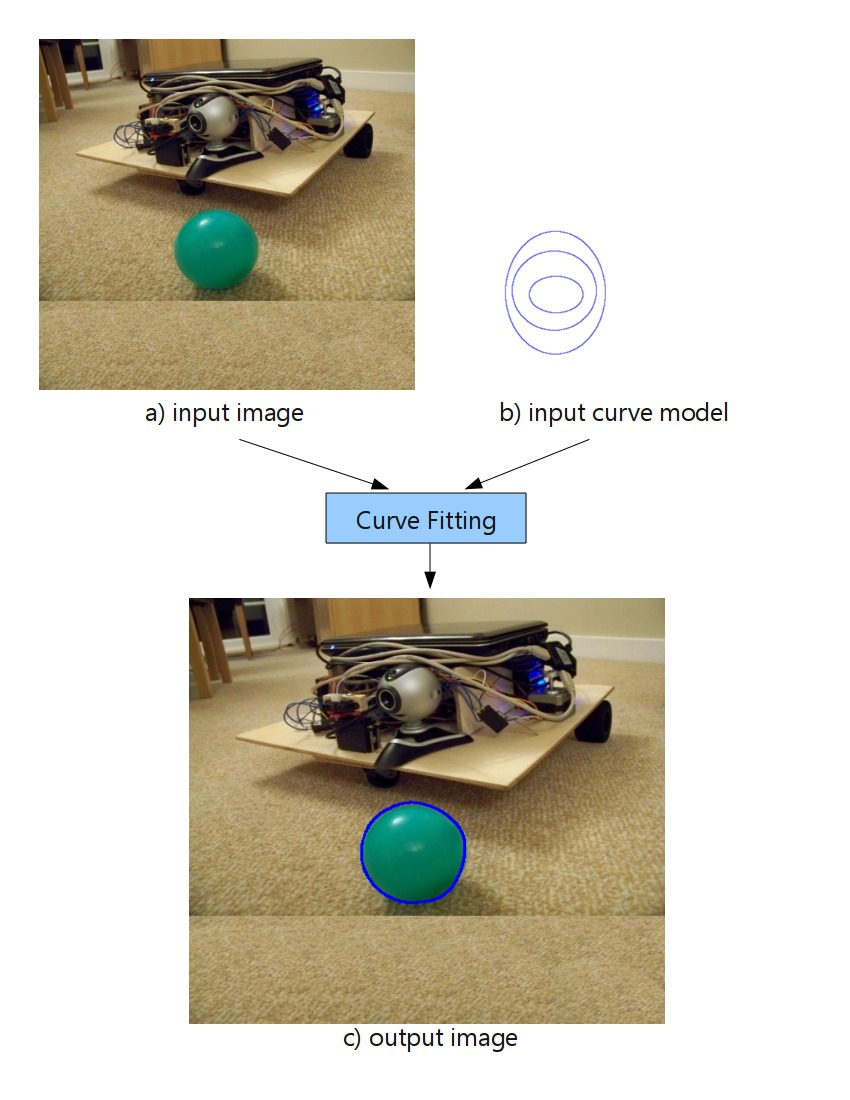
\includegraphics[width=10cm]{images/fitting.jpg}
  \caption[The description of curve-fitting problem]{a) an input
    image is given but not showing the pre-processing step. b) A series of
    parametric curve model contours which can be used to evaluate the
    prior distribution. These contours represent only a few possible
    shapes for the ball. c) The curve-fitting problem aims to estimate the model
    parameters by determining the posterior distribution. During the
    fitting process, the uncertainty of contours of the ball is widely
    reduced.}
  \label{fig:fitting}
\end{figure}

\section{Motivation For the CCD Algorithm}
\label{sec:mccd}
The curve-fitting problem and its variants have a wide range of
applications in the field of robotics, medical processing, user
interface, surveillance and biometrics~\cite{hanek2004fitting}. In order to be
widely applicable to practical personal robotics problems (such as
perception of mobile manipulation), robustness,
accuracy, efficiency and versatility should be
considered when a novel approach is designed and implemented.
However, in the computer vision community, solving object segmentation and the
related object contour tracking problems are always challenging,
especially in natural and unconstrained scenes. Due to clutter,
shading, texture, and highlights it is very difficult to segment
an object from an inhomogeneous background. Furthermore, some physical
conditions, such as the illumination or surface properties, will
influence the efficiency and stability of related approaches. It is
necessary and significant to develop a method which determines adequate segmentation
in advance or a single criterion that is applicable for all parts of objects boundaries.

Among the currently available methodologies, the CCD algorithm is
thought as the one that solves above problems best due to a high level
of robustness and sub-pixel accuracy even in the presence of severe
texture, shading, clutter, partial occlusion, and strong changes of
illumination and versatility. It is developed and presented as a state-of-the-art
improvement over other advanced techniques such as the condensation
algorithm~\cite{isard1998icondensation}. In the CCD approach, the curve-fitting problem is
put in the context of probabilistic framework and thus analogous to
the regression problem in the field of pattern recognition, which is especially
helpful to touch the nature of curve-fitting problem. By introducing
local image statistics, the algorithm can cope with highly
inhomogeneous image regions and provide therefore locally adapted
criteria for separating the adjacent image regions. The blurred
curve model is used as efficient means for iteratively optimizing the
posterior density over possible model parameters. It enables the
algorithm to trade-off two conflicting objectives, namely heaving a
large area of convergence and achieving high
accuracy~\cite{hanek2004fitting}.

The robustness, high performance and accuracy of the CCD algorithm enable it 
to be used on personal robot  because many applications in the field
of personal robotics are time-constrained. The object's contour
obtained by the CCD algorithm can be used to locate the object and 
establish a set of safe grasps on it~\cite{hanek2000vision}.

\section{The Contracting Curve Density (CCD) Algorithm}
\label{sec:sketch}

\subsection{An Alternative View of the CCD Algorithm}
\label{sec:overview}

In the field of pattern recognition, the key concept is that of
uncertainty. In image data, the uncertainty arises both
through noise from measurements, as well as through the nature of
the objects (e.g. cardiac motion and deformation). Probability theory
provides a consistent framework for the quantification and
manipulation of uncertainty.  In this section, we view curve-fitting
problem from a probabilistic perspective and turn us towards to
Bayesian logistic regression problem.

In the CCD algorithm, we aim to find the contour of observed object
and thus segment it from the background. Therefore, a hypothesis
contour divides the image into two part (Fig.\ref{fig:divide}), inside
and outside. For probabilistic model, we can represent this using
binary representation (e.g. $\{0, 1\}$). The goal of the CCD algorithm
is equivalent to accurately
assign a class label to each pixels in the image (Actually we only need assign those pixels in the vicinity of the
contour), thus the curve-fitting problem becomes a classification
one. A powerful approach to solve this problem involves modeling a
conditional probability distribution in an inference stage, and then
subsequently uses this distribution to make optimal decisions. In
order to derive the conditional probability, prior distribution and
likelihood function should be given.

\begin{figure}[htbp]
  \centering
    \begin{minipage}[t]{0.5\linewidth} 
    \centering 
        \subfloat[]{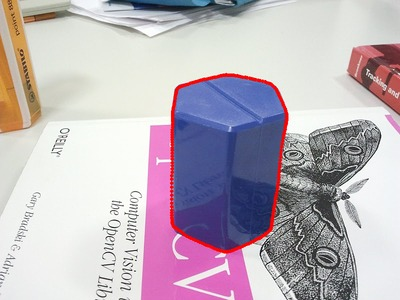
\includegraphics[width=8.0cm]{images/divide1.jpg}}
  \end{minipage}% 
  \begin{minipage}[t]{0.5\linewidth} 
    \centering 
    \subfloat[]{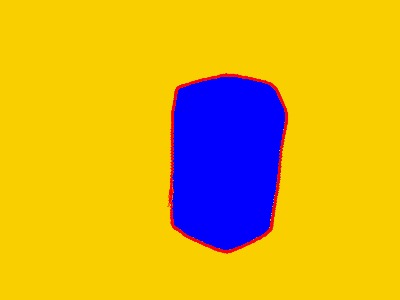
\includegraphics[width=8.0cm]{images/divide2.jpg}}
  \end{minipage} 
  \caption[A contour divide an image into two parts]{a) The red
    contour successfully segment the box from the background. b) The
    blue one is outside, the golden one is inside.}
  \label{fig:divide}
\end{figure}


We assume that a parametric curve model is governed by a prior distribution
over the model parameters (usually a multi-dimensional vector). There
exists a range of probability distributions which can be used to model
the distribution of shapes. In this thesis, for simplicity, let us
consider the Gaussian distribution, which is commonly used in computer
vison because of its several outstanding features. 


% \begin{equation}
%   \label{eq:1.1}
%   p(\mathbf{\Phi} | \mathbf{m}_{\mathbf{\Phi}}, \mathbf{\mathbf{\Sigma}}_{\mathbf{\Phi}}) = \mathcal{N}(\mathbf{\Phi} |
%   \mathbf{m}_{\mathbf{\Phi}},\mathbf{\Sigma}_{\mathbf{\Phi}}) =
%   \frac{1}{(2\pi )^{D/2}} \frac{1}{|\mathbf{\Sigma}_{\mathbf{\Phi}}|^{1/2}}
% \mathrm{exp} \left\{ -\frac{1}{2} (\mathbf{\Phi} -
%   \mathbf{\Sigma}_{\mathbf{\Phi}})^T \mathbf{\Sigma}_{\mathbf{\Phi}}^{-1} (\mathbf{\Phi} -
%   \mathbf{\Sigma}_{\mathbf{\Phi}}) \right\}
% \end{equation}
% where the $D$-dimensional vector $\mathbf{m}_{\mathbf{\Phi}}$ is
% called the mean, the $D \times D$ matrix
% $ \mathbf{\Sigma}_{\mathbf{\Phi}} $ is called
% the covariance, and $|\mathbf{\Sigma}_{\mathbf{\Phi}}|$ denotes the
% determinant of $\mathbf{\Sigma}_{\mathbf{\Phi}}$

%  Prior knowledge
% defines the possibility of a shape in an image, if we want to know what
% shape is presented in a given image, we must find the posterior
% distribution. 
Defining the prior distribution is only a step of the problem.
According to the Bayesian theorem, the conditional distribution
is proportional to the product of prior distribution and the likelihood
function. Hence, the next step is to define the likelihood function.

In the implementation of the CCD algorithm, it is suggested to use
local image pixels as the training data to determine the
likelihood function. If the data is assumed to be drawn  independently
from the distribution, then the likelihood function is given by the accumulation of all the components.
By pixel value we denote the vector containing the local single-or multichannel
image data associated to a pixel. In our experiments, we directly use the sensed RGB
values as pixel values. However, other types of local features computed in a pre-processing
step may also be used, e.g. texture descriptors or color values in
other color spaces.

The likelihood function obtained from the local statistics has
not a closed-form solution. In addition, the prior distribution is just
an approximate to the true distribution. Therefore, Maximization
likelihood method does not work here, we have to use an alternative
approach known as iterative reweighted least squares (IRLS) to find
the solution. Here the IRLS process is called Maximum a Posterior, or
simply MAP.

In the CCD algorithm, because we just need a parameter vector determining
the shape of specified contour, we do not plan to calculate the
predictive distribution. Therefore, the MAP solution mentioned above
is our objective.

However, take account into the fact that exact inference for the
regression is always intractable, we could encounter some issues before
implementing the algorithm. In the next section, we will discuss these
problems.

% According to the Bayesian treatment for regression, 
% With the prior distribution and posterior distribution, we can now
% apply the Bayesian theorem to the curve-fitting problem.
% We determine $\hat{\mathbf{\Phi}}$ by finding the most probable
% value of $\mathbf{\Phi}$ given by the data, in other words by maximizing
% the posterior distribution. This technique is called maximum
% posterior, or simply MAP.

% There are several methods to estimate the MAP~\cite{map}:
% \begin{itemize}
% \item In some special cases, posterior distribution can be given in
%   closed form analytically. This requires conjugate priors.
% \item Numerical optimization such as the conjugate gradient method or
%   Newton's method.
% \item Modification of an expectation-maximization (EM) algorithm,
%   which does not require to derive the posterior density.
% \item Monte Carlo method using simulated annealing.
% \end{itemize}

% In this thesis, we adopt the second method to obtain the MAP estimate.
% Usually, the results are some parameters (e.g. mean and covariance) to
% govern the posterior distribution. With the resulting parameters we
% can predict what shape is actually likely to be present in a particular image.

\subsection{Improvements Based on the Original CCD Algorithm}
\label{sec:prob}
Some key issues have been explained in the origin
implementation~\cite{hanek2004contracting}.
After evaluating the CCD algorithm, some new questions are posed.

\begin{itemize}
\item How to create a parametric curve model as prior knowledge and
  make it well approximate the distribution of contour shapes? 
There are a variety of active shape models available, such as principally snakes,
  deformable templates and dynamic contours. For curve-fitting
  problem, deformable template is a good choice to match the image
  data. Model parameters control the complexity of parametric curve,
  as well degrees of freedom. There is a trade-off between the degree
  of contour and complexity, with very flexible models having high
  computational cost and design barrier, and relatively rigid models
  having low accuracy and high misclassification rate. 

\item Moreover, one
  main limitation of the CCD algorithm is manual initialization. How can
  we avoid too much manual intervention?

\item How can the local statistics in the image be efficiently
  evaluated? First, it is necessary to establish the relation between the model parameters
  and the image data. This is especially challenging in the presence
  of clutter and strong texture if we consider the factors, such as
  illumination, surface properties, characteristics of the camera and
  shadow. 

\item How can the fit be optimized efficiently? Many
  nonlinear optimization algorithms used to estimate MAP could find
  multiple local maxima and  are not guaranteed to find the largest
  out of these maxima.
\end{itemize}

Based on these questions, we improve the CCD algorithm from the
following aspects:
\begin{itemize}
\item We will use parametric B-Spline curve as
parametric model curve. It is proved that this type of curve model is
flexible enough and can well represent the contour of the
object. Both 6-D and 8-D model parameters vector
are provided in our implementation. The parametric model with 8
degrees of freedom can efficiently fit objects in non-planar affine
space. Parametric B-Spline curve will be described in
Chapter~\ref{chapter:bspline}.
\item In order to avoid human intervention, we add a feature to 
  initialize a contour from Scale-invariant feature transform (SIFT)
  features or a point cloud polygon.
\item The local statistics is the main feature of the CCD
  algorithms. The blurred curve models can considerably decrease the
  computational cost. However, excessive sparse samples may ignore some
  features in the vicinity of the curve. Hence, before we blur the
  model, we compute the circumference of a contour thus reasonably
  sample pixels from the vicinity of the curve.
\item Experiments show that the probit regression function used
  in original implementation is sensitive to outliers. In this
  thesis, we make it support both probit and logistic regression
  function.
\item We have used some new optimization methods instead of the
  newton method, such as least squares support vector machine.
\end{itemize}

% The second question is especially challenging. In order to simplify
% the problem, it is necessary to make some assumptions about the image
% data. We will describe such assumptions in more detail. For the last
% question, different optimization methods used for curve-fitting will
% be discussed in this thesis.

Moreover, in order to deploy the CCD algorithm in personal robotics,
we have to scale the algorithm and implement it using OpenCV library.
The algorithm will be released under the open source BSD license. Some
related information can be found on\\
\url{http://www.ros.org/wiki/contracking\_curve\_density\_algorithm}

\subsection{Sketch of the CCD algorithm}
\label{sec:sccd}

In this section, the basic steps of the CCD algorithm will be
sketched. 
\begin{enumerate}
\item \textbf{Initialization}: Given an input image as training data, we first choose an initial
contour for an object or feature which will be fitted or tracked, and
some initial values for the means, covariances. For most practical
application, pre-processing stage is necessary to make the problem
easier to solve. 
\item \textbf{Local statistics}: In the step of learning local
  statistics, for each pixel in the
vicinity of the expected curve, two sets of local statistics
are computed, one set for each side of the curve. The local statistics are obtained from
pixels that are close to the pixel on the contour and most likely lie
on the corresponding side of the curve, according to the current
estimate of the model parameters. The resulting local statistics
represent an expectation of "what the two sides of the curve look
like"~\cite{hanek2004contracting}, which is known as likelihood.
\item \textbf{Refining parameters}: The conditional distribution, namely
  the product of prior distribution and  the likelihood, is evaluated
  as the cost function. Then MAP estimate is executed to optimize the
  parameters, as a result, MAP value of model parameters vector and
  covariance will be given in this step.
\item \textbf{Checking Convergence}: Check for convergence of either
  the parameters or log cost function. If the convergence criterion is
  not satisfied return to step 2.
\end{enumerate}
Fig.\ref{fig:flowchart} gives the flow chart of the CCD algorithm.
\begin{figure}[htb]
  \centering
  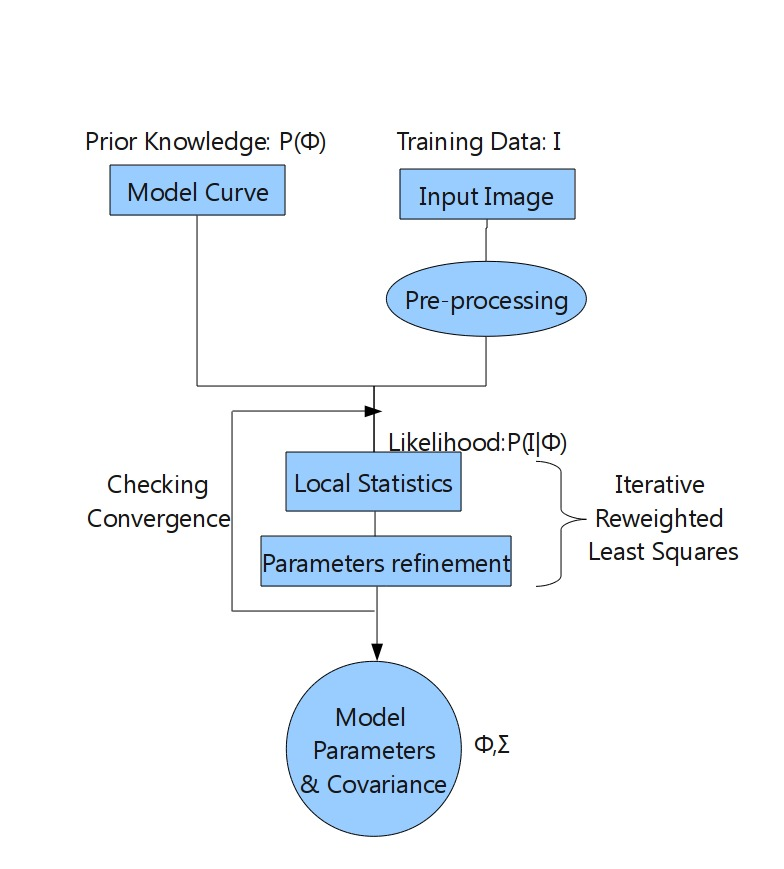
\includegraphics[width=10cm]{images/flowchart.jpg}
  \caption[The flow chart of
  the CCD algorithm ]{The flow chart of the CCD algorithm}
  \label{fig:flowchart}
\end{figure}


% The CCD algorithm has some interesting similarities to the Expectation-Maximization
% (EM) algorithm (Dempster et al., 1977), which is often used for clustering-based image
% segmentation, a subset of region-based image segmentation (Hermes et al., 2002; Belongie
% et al., 1998). The first step computes local statistics defining an expectation of the pixel
% values (E-step). The second step maximizes this expectation
% (M-step). The CCD algorithm differs mainly by: 1.) using local
% statistics, 2.) exploiting a curve model and optimizing model
% parameters rather than pixel classifications.


\section{Overview of the Thesis}
\label{sec:overview}
The remainder of the work at hand is organized as
follows. Chapter~\ref{chapter:related} describes the related work on
active contour, model-based image segmentation and tracking, as well
as optimization methods. In Chapter~\ref{chapter:SHI}, we give a brief introduction of software
and hardware infrastructure used in the implementation of the CCD
approach. We will concern the OpenCV library, ROS and PR2. Details on shape-space models and parametric
B-Spline curves are discussed in Chapter~\ref{chapter:bspline},  and
Chapter~\ref{chapter:ccd} explains the CCD approach in detail. 
In Chapter~\ref{chapter:experiments}, experiments and results are demonstrated.%  In
% addition, we evaluate the performance of the CCD algorithm and the CCD
% tracker in terms of robustness, accuracy, and runtime.
In Chapter~\ref{chapter:conclusion},
the work of this thesis is concluded with the future work for improvement.



